\documentclass[conference]{IEEEtran}
\usepackage[utf8]{inputenc}
\usepackage[T1]{fontenc}
\usepackage{graphicx,amsmath,array,booktabs,xcolor,listings,url,microtype}
\usepackage[hidelinks]{hyperref}
\hypersetup{pdftitle={Control de un UR5 con pinza paralela en ROS 2 y MoveIt},pdfauthor={Brayan Mateo Bravo Losada}}
\renewcommand{\abstractname}{Resumen}
\renewcommand{\IEEEkeywordsname}{Palabras clave}
\renewcommand{\refname}{Referencias}
\renewcommand{\figurename}{Fig.}
\renewcommand{\tablename}{TABLA}
\renewcommand{\lstlistingname}{Código}
\definecolor{codegray}{RGB}{247,247,247}
\lstset{basicstyle=\ttfamily\scriptsize,backgroundcolor=\color{codegray},
 frame=single,rulecolor=\color{gray},breaklines=true,columns=fullflexible,
 keepspaces=true,showstringspaces=false,captionpos=b}
\urlstyle{tt}
\emergencystretch=1em
\graphicspath{{figuras/}}
\newcommand{\laburl}{https://github.com/Mate02010/rospart3/tree/main/laboratorios/ur5_gripper}
\newcommand{\filelab}{https://github.com/Mate02010/rospart3/blob/main/laboratorios/ur5_gripper}
\newcommand{\rawlab}{https://raw.githubusercontent.com/Mate02010/rospart3/refs/heads/main/laboratorios/ur5_gripper}
\title{Control de un UR5 con pinza paralela en ROS 2\\
y planificación de trayectorias con MoveIt}
\author{\IEEEauthorblockN{Brayan Mateo Bravo Losada}
\IEEEauthorblockA{Ingeniería Electrónica\\
Escuela Colombiana de Ingeniería Julio Garavito\\
Robótica -- Corte 2, Práctica 2\\
Bogotá, Colombia}}
\begin{document}
\maketitle

\begin{abstract}
Se integró un manipulador UR5 con una pinza paralela de dos dedos en un
workspace ROS 2 Kilted y se verificó su funcionamiento en Gazebo Sim.
Se implementó una rutina de recogida y colocación con cuatro objetivos
articulares diferentes, apertura y cierre, mensajes informativos y señales
digitales simuladas. La secuencia se ejecutó por tópicos y mediante MoveIt.
Además, se generó una configuración con la interfaz gráfica de MoveIt Setup
Assistant y se probaron los grupos del brazo y de la pinza en RViz.
Las dos ejecuciones registradas completaron ocho movimientos cada una.
Se conservaron mediciones articulares, capturas y cuatro videos.
El brazo y los dedos se simulan físicamente; la pieza se representa
mediante estados lógicos, sin acreditar agarre por contacto.
\end{abstract}
\begin{IEEEkeywords}
UR5, ROS 2, Gazebo Sim, MoveIt, Setup Assistant, pinza paralela,
pick and place.
\end{IEEEkeywords}

\section{Introducción}
La práctica propone construir los paquetes de un UR5 con gripper,
identificar sus interfaces de control e implementar una rutina de
\textit{pick and place}. También exige generar una configuración propia
de MoveIt, comprobarla desde RViz y utilizarla desde un nodo.
El punto de partida fue el repositorio del profesor
\texttt{ur5\_gripper\_packages}~\cite{teacher}, conservando la revisión
\texttt{87a547dfde78} como referencia del código base.

El objetivo fue verificar la integración entre descripción del robot,
controladores, simulación y planificación. La existencia de un comando
publicado no se tomó como prueba suficiente de movimiento: la aplicación
comprueba posiciones articulares medidas y, en el modo MoveIt, el resultado
de la planificación y de la ejecución. Las evidencias corresponden a esta
práctica y no reutilizan las trayectorias de la práctica anterior de URSim.

\section{Arquitectura del sistema}
\subsection{Entorno y organización}
Se reutilizó el entorno del equipo: Windows, Ubuntu 24.04 mediante WSL2,
ROS 2 Kilted, Gazebo Sim Ionic 9.5.0, MoveIt 2 y
\texttt{gz\_ros2\_control}. La documentación de ROS y Gazebo se usó como
referencia de la preparación del entorno~\cite{ros,rosgazebo}.
No se reinstalaron estos componentes para producir la solución.

La práctica se organiza en cuatro paquetes.
\texttt{ur5\_robotiq\_description} contiene los Xacro del brazo y la
pinza; \texttt{ur5\_robotiq\_bringup} inicia el mundo y los controladores;
\texttt{lab\_manipulador} implementa la secuencia y las señales
digitales; y \texttt{ur5\_gripper\_moveit} contiene SRDF, cinemática,
límites, planificador, controladores y configuración de RViz.
Los nombres conservan la base docente, pero la pinza utilizada es el
modelo geométrico paralelo de dos articulaciones prismáticas.

Los paquetes están directamente en la carpeta de la práctica, junto al
README y al lanzador \texttt{ejecutar.sh}. En \texttt{evidencias/} se reúnen
el informe, sus fuentes LaTeX, los videos y los resultados de las pruebas.
Las carpetas de compilación y las evidencias de nuevas ejecuciones
se generan localmente y se excluyen de Git.

\begin{figure*}[t]
\centering
\setlength{\tabcolsep}{3pt}
\begin{tabular}{c@{\quad$\longrightarrow$\quad}c@{\quad$\longrightarrow$\quad}c@{\quad$\longrightarrow$\quad}c}
\fbox{\shortstack{Aplicación\\\texttt{pick\_place}}}&
\fbox{\shortstack{Tópicos ROS\\o MoveIt}}&
\fbox{\shortstack{Controladores\\de brazo y pinza}}&
\fbox{\shortstack{Gazebo\\UR5 y dedos}}
\end{tabular}
\par\smallskip
\small Realimentación mediante \texttt{/joint\_states} y sincronización con
\texttt{/clock}. El nodo \texttt{digital\_io} simula las señales de la celda.
\caption{Arquitectura de las dos vías de ejecución. MoveIt entrega
trayectorias a los mismos controladores utilizados por Gazebo.}
\label{fig:architecture}
\end{figure*}

\subsection{Interfaces de control}
El brazo utiliza el controlador
\path{scaled_joint_trajectory_controller}. La pinza se configuró con
\texttt{JointTrajectoryController} para sus dos dedos. Ambos reciben mensajes de tipo
\path{trajectory_msgs/msg/JointTrajectory}.
Los dos controladores ofrecen la acción
\texttt{FollowJointTrajectory} para ejecutar desde MoveIt.
Los tópicos directos son:
\begin{itemize}
\item \path{/scaled_joint_trajectory_controller/joint_trajectory}.
\item \path{/gripper_controller/joint_trajectory}.
\end{itemize}
Los estados se obtienen de \path{/joint_states}, de tipo
\texttt{sensor\_msgs/msg/JointState}. Las posiciones de las seis
articulaciones del brazo se expresan en radianes y las de los dedos
prismáticos, en metros.

La entrada y salida digitales utilizan
\path{/lab/digital_input} y \path{/lab/digital_output}, de tipo
\texttt{std\_msgs/msg/Bool}. El servicio
\path{/lab/set_digital_input}, de tipo
\texttt{std\_srvs/srv/SetBool}, cambia manualmente la entrada.
El tópico \path{/lab/waiting_input} informa que la secuencia está
bloqueada, mientras \path{/lab/status} publica sus eventos como JSON.

\section{Metodología}
\subsection{Construcción y comprobación inicial}
Primero se inspeccionaron el modelo, las articulaciones y los
controladores del repositorio base. Después se construyeron los paquetes
con \texttt{colcon} y se inició Gazebo con un solo gestor de control.
El dominio ROS utilizado fue 74 y los nodos que consumen el estado de
la simulación compartieron su reloj.

Se comprobaron comandos del brazo y de la pinza antes de ejecutar la
rutina completa. El siguiente ejemplo corresponde al cierre de los dedos:
\begin{lstlisting}[language=bash,caption={Comando directo de cierre de la pinza.}]
ros2 topic pub --once \
 /gripper_controller/joint_trajectory \
 trajectory_msgs/msg/JointTrajectory \
 "{joint_names: [gripper_finger_joint,
 right_finger_joint], points: [{
 positions: [0.004, 0.004],
 time_from_start: {sec: 1}}]}"
\end{lstlisting}
El README conserva también el comando del brazo y la apertura de la
pinza. Se emplean posiciones de $0.04$ m en apertura y $0.004$ m
en cierre para cada dedo; estos valores no son una medición de fuerza
ni una prueba de sujeción de una pieza.

\subsection{Criterio de verificación}
Para cada grupo se calculó el error final
\begin{equation}
 e_{\max}=\max_i\left|q_i^{\mathrm{medido}}-q_i^{\mathrm{objetivo}}\right|.
 \label{eq:error}
\end{equation}
El nodo exige error menor que $0.02$ rad para el brazo y $0.002$ m
para los dedos durante cuatro actualizaciones consecutivas.
El registro \texttt{motion\_success} guarda el error observado al
declarar completado ese movimiento. Los máximos de este informe se
calculan sobre dichos registros; no representan el máximo error
instantáneo de toda la trayectoria.

En el modo MoveIt se comprueba además el código de respuesta de
\texttt{GetMotionPlan}, la aceptación de \texttt{ExecuteTrajectory}
y su resultado final. La prueba solo se considera exitosa cuando
la secuencia completa termina sin excepción y guarda
\texttt{success: true}.

\section{Implementación de la rutina}
\subsection{Objetivos articulares y operaciones}
Se definieron cuatro objetivos diferentes para el brazo, en el orden
\[
 \mathbf q=[q_{\mathrm{pan}},q_{\mathrm{lift}},q_{\mathrm{elbow}},
 q_{\mathrm{w1}},q_{\mathrm{w2}},q_{\mathrm{w3}}].
\]
La Tabla~\ref{tab:poses} resume sus posiciones. La secuencia comienza en
Preparación y retorna a ese punto al finalizar; por tanto, se ejecutan
cinco movimientos del brazo, pero solo cuatro objetivos distintos.

\begin{table}[t]
\caption{Objetivos del brazo utilizados en la rutina, en radianes}
\label{tab:poses}
\centering
\scriptsize
\begin{tabular}{@{}lp{0.73\columnwidth}@{}}
\toprule
Punto & Vector objetivo\\
\midrule
Preparación & $[0,-1.57,1.57,-1.57,-1.57,0]$\\
Recogida & $[0.35,-1.45,1.80,-1.92,-1.57,0]$\\
Intermedio & $[0,-1.20,1.40,-1.77,-1.57,0]$\\
Entrega & $[-0.40,-1.45,1.80,-1.92,-1.57,0]$\\
\bottomrule
\end{tabular}
\end{table}

En Preparación se emite el mensaje de inicio y se abre la pinza.
En Recogida se cierra y se registra el estado lógico de pieza recogida.
En Intermedio se activa la salida digital. En Entrega se abre la pinza,
se registra la liberación y se espera la confirmación digital.
Tras recibirla se desactiva la salida y se retorna a Preparación.

El orden del código conserva estas operaciones de forma explícita:
\begin{lstlisting}[language=Python,caption={Fragmento de la operación en Intermedio y Entrega.}]
self.move('arm', ARM, POSES['Intermedio'],
          'Intermedio')
self.digital_out.publish(Bool(data=True))
self.move('arm', ARM, POSES['Entrega'],
          'Entrega')
self.gripper(True)
self.waiting_out.publish(Bool(data=True))
\end{lstlisting}
El código completo añade eventos, comprobaciones y manejo de errores.
Las tres operaciones de la pinza, sumadas a los cinco movimientos
del brazo, explican los ocho movimientos registrados por ejecución.

\subsection{Entrada digital y sincronización}
La espera requiere observar una entrada BAJA seguida de una nueva
entrada ALTA. El contador de mensajes evita aceptar como confirmación
un estado ALTO anterior al comienzo de la espera. No se trata de una
entrada eléctrica de hardware.

El nodo \texttt{digital\_io} permite dos modos. En el manual, el usuario
llama al servicio \texttt{SetBool}. En el automático se genera la
misma transición después de 1.5 s para que la demostración pueda
repetirse. Las grabaciones finales utilizaron este segundo modo.
Las órdenes manuales equivalentes son:
\begin{lstlisting}[language=bash,caption={Confirmación digital simulada.}]
ros2 service call /lab/set_digital_input \
 std_srvs/srv/SetBool "{data: false}"
ros2 service call /lab/set_digital_input \
 std_srvs/srv/SetBool "{data: true}"
\end{lstlisting}

\section{Configuración y ejecución con MoveIt}
\subsection{Generación mediante Setup Assistant}
Se utilizó la interfaz gráfica de MoveIt Setup Assistant
2.14.3~\cite{setup}. Se cargó el modelo
\path{ur_with_gripper_moveit.urdf.xacro}, que integra el brazo y la
pinza, y se generó la matriz de autocolisiones con 10\,000 muestras.
El paquete se produjo mediante la opción de generación de archivos
del asistente, como muestra la Fig.~\ref{fig:assistant}.

\begin{figure}[t]
\centering
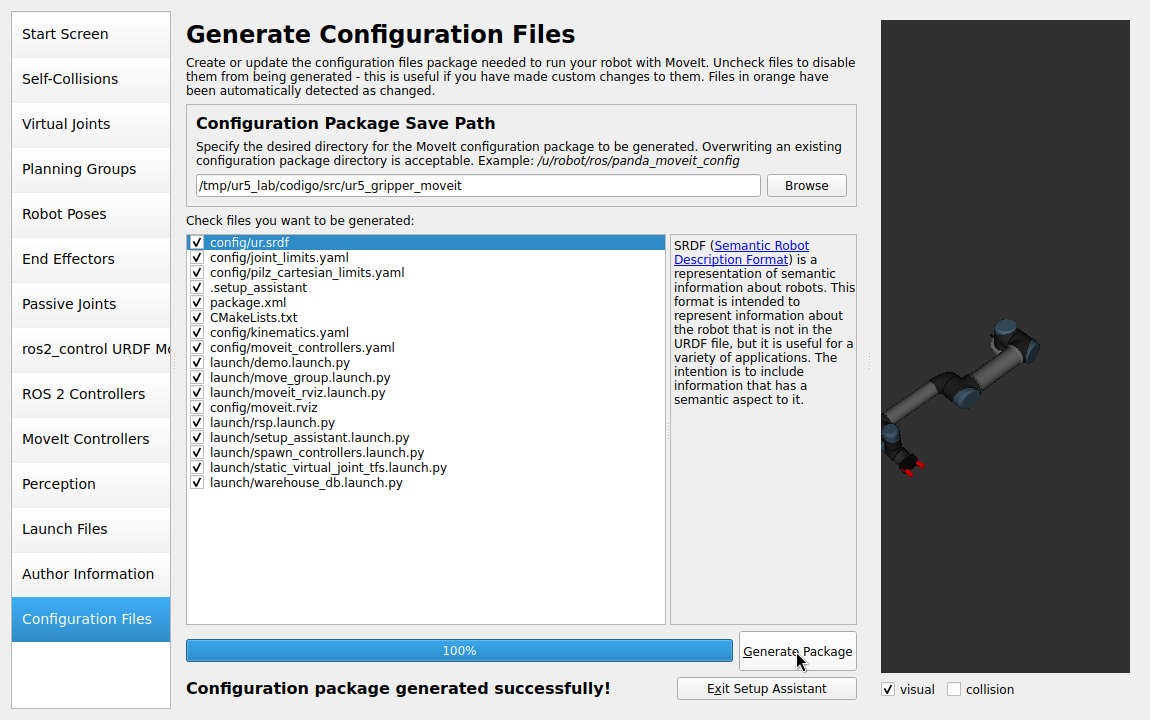
\includegraphics[width=\columnwidth]{07_paquete_generado.png}
\caption{Generación del paquete en Setup Assistant. El mensaje de
finalización acredita la generación mediante la interfaz gráfica;
el proceso está documentado en el video 01.}
\label{fig:assistant}
\end{figure}

Se configuró el grupo \texttt{arm} como cadena
\texttt{base\_link}--\texttt{tool0}, con el solucionador cinemático KDL.
El grupo \texttt{gripper} contiene
\texttt{gripper\_finger\_joint} y
\texttt{right\_finger\_joint}. El efector \texttt{eef} se monta
en \texttt{tool0} y utiliza el grupo de pinza, con \texttt{arm}
como grupo padre. El URDF ya contiene una unión fija con
\texttt{world}; no se añadió una referencia fija redundante.

Después de la generación se alinearon los nombres de controladores
con Gazebo, se añadieron los estados nombrados del brazo y los estados
\texttt{Open}/\texttt{Close}, y se configuraron los límites de
aceleración y OMPL/RRTConnect. Estos ajustes no sustituyen la
generación inicial por interfaz gráfica. El SRDF y el archivo
\texttt{.setup\_assistant} se conservan dentro del paquete.

\subsection{Planificación desde un nodo}
El modo \texttt{moveit} usa el servicio
\path{/plan_kinematic_path}, de tipo
\texttt{moveit\_msgs/srv/GetMotionPlan}, y la acción
\path{/execute_trajectory}, de tipo
\texttt{moveit\_msgs/action/ExecuteTrajectory}.
El estado inicial procede de \texttt{/joint\_states}; las metas se
expresan como restricciones articulares del grupo seleccionado.

Cada solicitud utiliza el pipeline \texttt{ompl}, el planificador
\texttt{RRTConnect}, hasta cinco intentos, cinco segundos de tiempo
de planificación permitido y factores de velocidad y aceleración de
$0.3$. Las tolerancias de las restricciones articulares se fijan en
$0.001$ en la unidad correspondiente a cada joint.
Los cinco segundos son un límite configurado por consulta, no el
tiempo medido de todas las planificaciones.

\begin{lstlisting}[language=Python,caption={Configuración de la solicitud de planificación.}]
plan.group_name = group
plan.pipeline_id = 'ompl'
plan.planner_id = 'RRTConnect'
plan.allowed_planning_time = 5.0
plan.num_planning_attempts = 5
plan.max_velocity_scaling_factor = 0.3
plan.max_acceleration_scaling_factor = 0.3
\end{lstlisting}
El lanzador \texttt{gazebo\_moveit.launch.py} inicia MoveIt y RViz
sobre la simulación ya activa. Utiliza los mismos controladores
y no inicia otro gestor de hardware.

\section{Validación y resultados}
\subsection{Pruebas de los grupos en RViz}
En el plugin MotionPlanning se seleccionó el grupo \texttt{arm},
el inicio \texttt{<current>} y el objetivo \texttt{Recogida}.
Se pulsó \textit{Plan}, se revisó la trayectoria y después
\textit{Execute}. La consulta registrada tardó aproximadamente
$0.079$ s en planificar y terminó con ejecución \texttt{SUCCEEDED}.
Se repitió el procedimiento con \texttt{gripper} y el objetivo
\texttt{Close}; la planificación tardó aproximadamente $0.062$ s
y la ejecución también finalizó correctamente.

\begin{figure}[t]
\centering
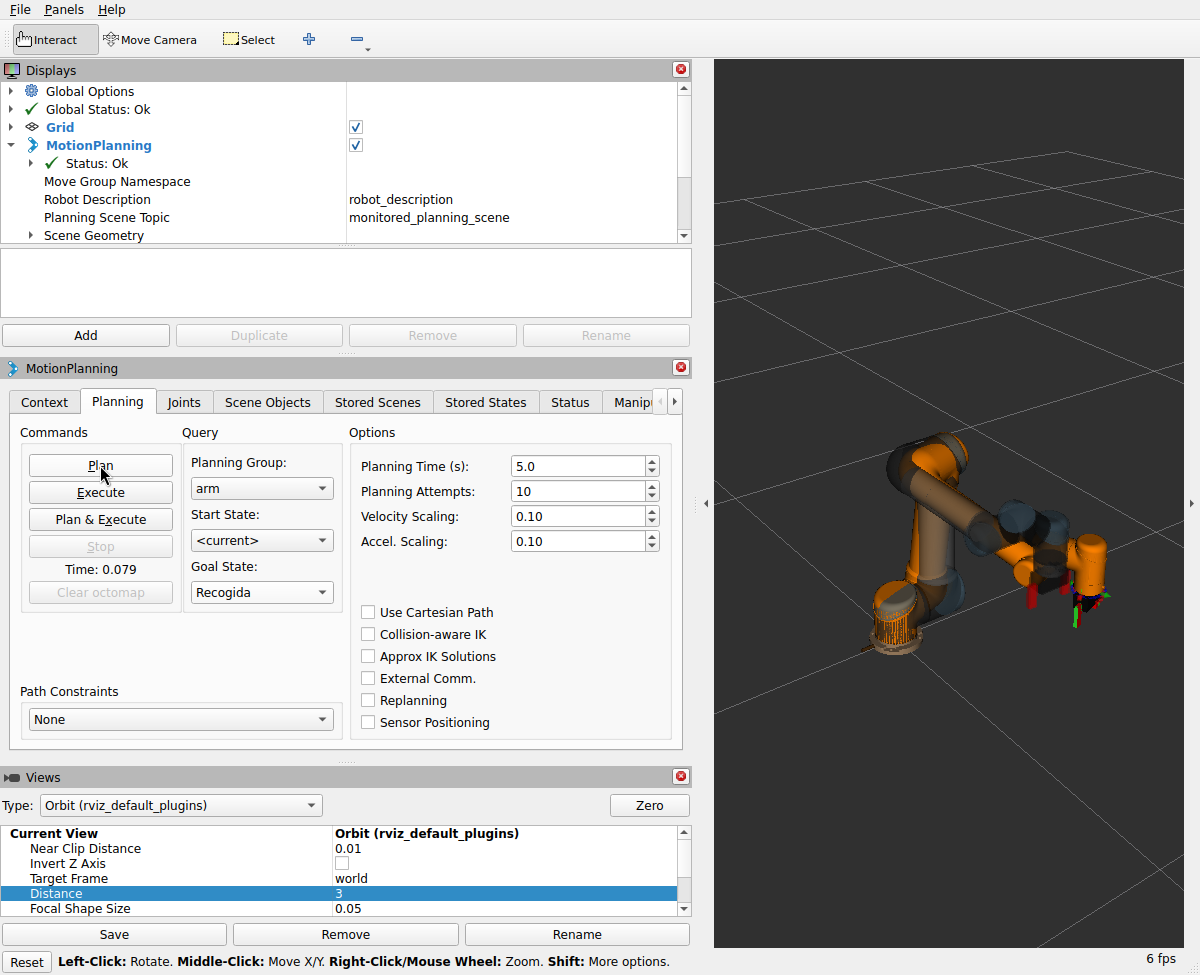
\includegraphics[width=\columnwidth]{10_rviz_plan_brazo.png}
\caption{Consulta de planificación del brazo en RViz, con objetivo
Recogida. El video 02 permite revisar la selección del grupo y
la posterior ejecución.}
\label{fig:rviz_arm}
\end{figure}
\begin{figure}[t]
\centering
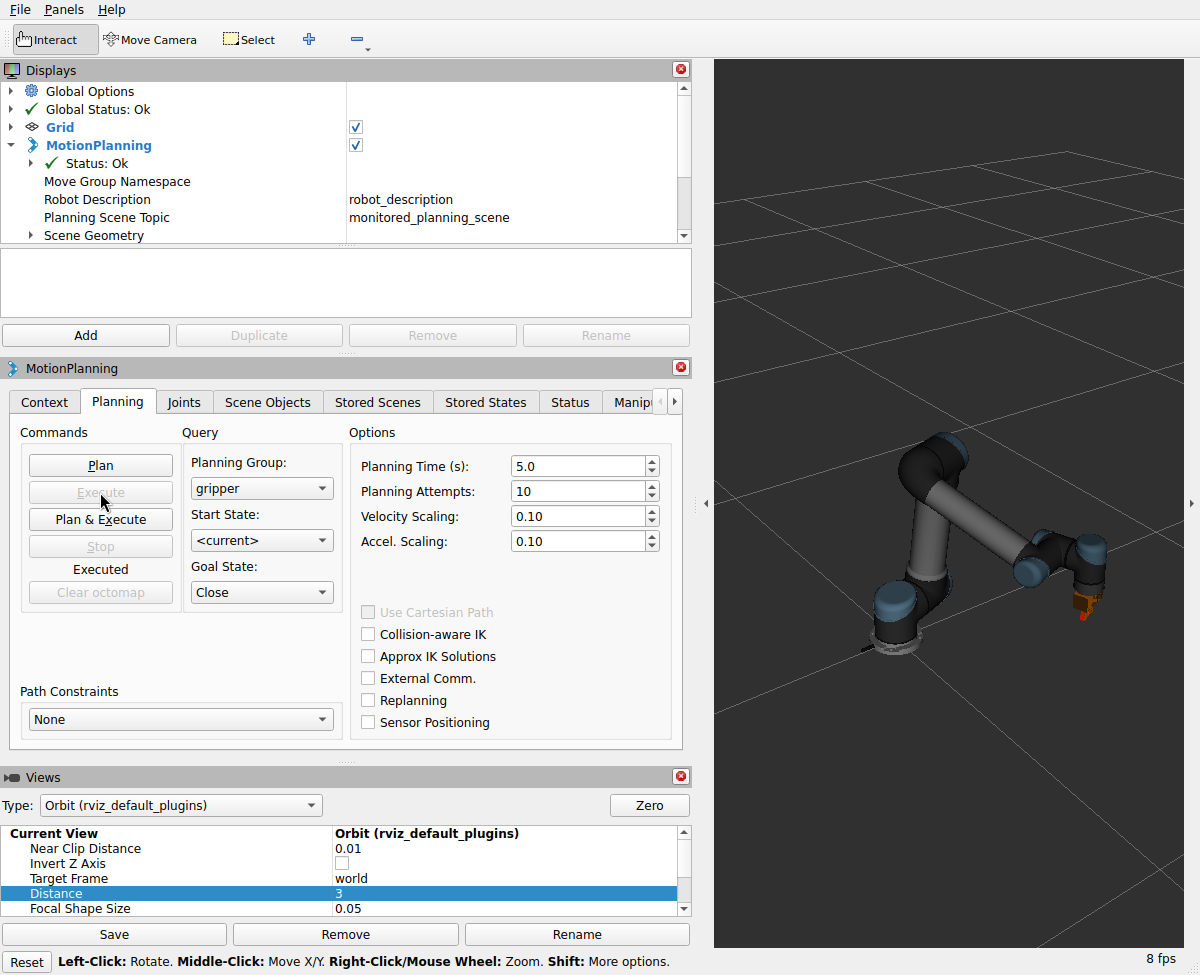
\includegraphics[width=\columnwidth]{16_rviz_gripper_completado.png}
\caption{Prueba del grupo gripper y ejecución completada desde
MotionPlanning. Esta comprobación es independiente de la rutina
automática ejecutada por el nodo.}
\label{fig:rviz_gripper}
\end{figure}

\subsection{Rutinas completas}
Los cuatro paquetes finalizaron su compilación. Las dos ejecuciones
grabadas terminaron con \texttt{success: true}, ocho movimientos y
confirmación digital. El modo MoveIt registró además ocho eventos
de planificación exitosa. La Tabla~\ref{tab:results} resume
las mediciones de los JSON.

\begin{table}[t]
\caption{Resultados de las ejecuciones registradas}
\label{tab:results}
\centering
\scriptsize
\setlength{\tabcolsep}{3pt}
\begin{tabular}{@{}lcc@{}}
\toprule
Medida & Tópicos ROS & Nodo MoveIt\\
\midrule
Movimientos completados & 8/8 & 8/8\\
Objetivos distintos del brazo & 4 & 4\\
Planes exitosos de MoveIt & No aplica & 8/8\\
Máx. error final brazo [rad] & 0.019704 & 0.000937\\
Máx. error final dedos [m] & 0.001949 & 0.000949\\
Tiempo de rutina [s] & 70.9 & 53.5\\
Confirmación digital & Recibida & Recibida\\
\bottomrule
\end{tabular}
\end{table}

Los tiempos corresponden al reloj de pared entre el primer y el
último evento de la rutina, incluyendo la espera digital. No son
duraciones de simulación ni la duración total del archivo de video,
que incluye preparación y cierre de la grabación.
Los resultados incluyen objetivos, eventos y muestras de estados
articulares para comprobar los valores de la tabla.

\begin{figure}[t]
\centering
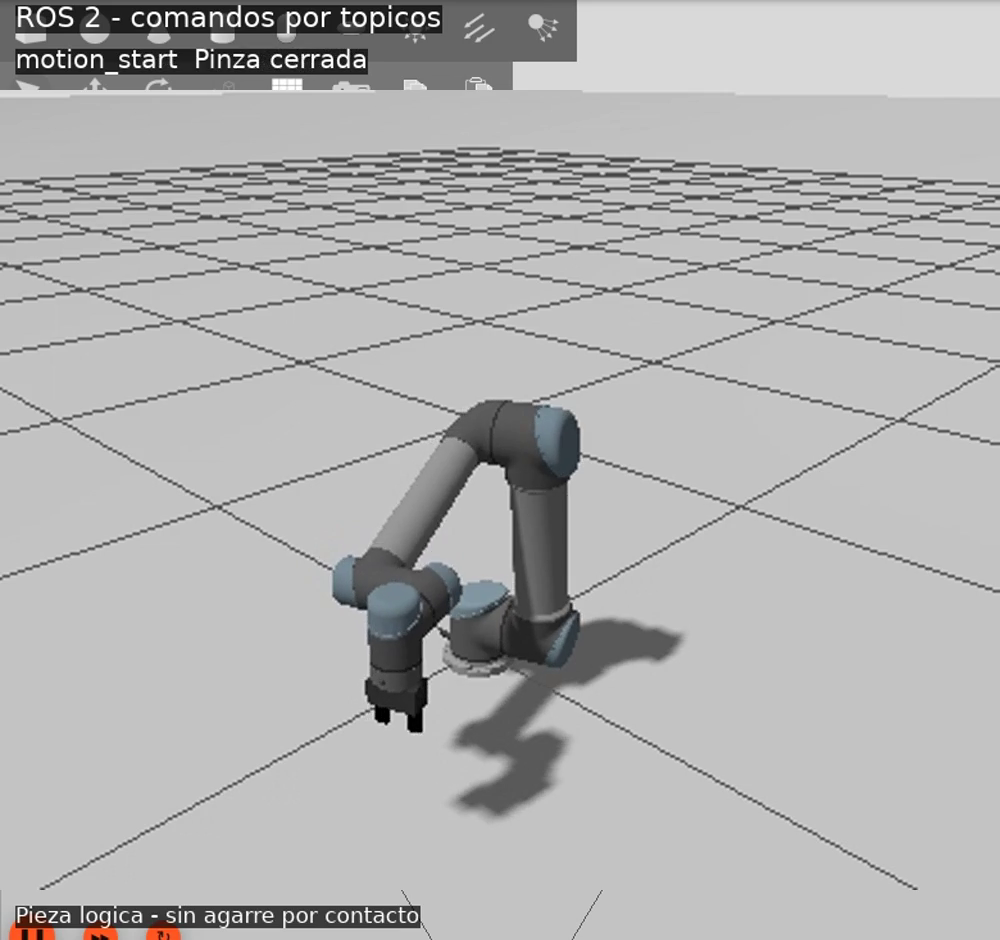
\includegraphics[width=\columnwidth]{21_gazebo_topics.png}
\caption{UR5 y pinza articulada durante la rutina por tópicos.
Fotograma del video 03, con el robot y sus eventos visibles.
Los videos 03 y 04 conservan las secuencias completas en tiempo real.}
\label{fig:gazebo}
\end{figure}

\subsection{Recursos y reproducción}
La solución está disponible en
\href{\laburl}{la carpeta del laboratorio en rospart3}~\cite{solution}.
Los accesos principales son:
\begin{itemize}
\item \href{\laburl/lab_manipulador}{Paquete de la aplicación Pick and Place}.
\item \href{\laburl/ur5_gripper_moveit}{Configuración generada de MoveIt}.
\item \href{\laburl/evidencias/resultados}{Resultados medidos de las pruebas}.
\item \href{\laburl/evidencias/informe}{Proyecto LaTeX para Overleaf}.
\end{itemize}
El índice \href{\filelab/evidencias/VIDEO.md}{\texttt{evidencias/VIDEO.md}} reúne los
cuatro videos, que también pueden descargarse directamente:
\begin{enumerate}
\item \href{\rawlab/evidencias/videos/01_setup_assistant_resumen.mp4}{Setup Assistant},
117.7 s, reproducción acelerada $\times8$.
\item \href{\rawlab/evidencias/videos/02_rviz_grupos_resumen.mp4}{Pruebas de RViz},
112.6 s, reproducción acelerada $\times4$.
\item \href{\rawlab/evidencias/videos/03_topics_gazebo.mp4}{Rutina por tópicos},
99.0 s, tiempo real.
\item \href{\rawlab/evidencias/videos/04_moveit_gazebo.mp4}{Rutina por MoveIt},
81.6 s, tiempo real.
\end{enumerate}
La aceleración se declara en los dos videos de interfaz. Las rutinas
mantienen su tiempo real; la pieza permanece identificada como lógica.

Para reproducir la práctica se compilan los paquetes desde su carpeta.
En terminales distintas se mantienen simulación, señales digitales
y planificador. Una cuarta terminal ejecuta una sola rutina a la vez:
\begin{lstlisting}[language=bash,caption={Arranque, con un proceso por terminal.}]
bash ejecutar.sh build
# Terminales independientes:
bash ejecutar.sh sim true
bash ejecutar.sh io true
bash ejecutar.sh planificador
# Otra terminal, elegir un modo:
bash ejecutar.sh topics
bash ejecutar.sh moveit
\end{lstlisting}
Los dos últimos comandos son alternativas secuenciales y no deben
iniciarse al mismo tiempo. El README detalla la preparación de
terminales para los comandos ROS manuales.

\section{Análisis de resultados}
Las pruebas por tópicos y mediante MoveIt verifican dos niveles
diferentes. La primera vía comprueba el formato del comando, los
suscriptores de los controladores y la llegada al objetivo. La segunda
añade generación de una trayectoria y comprobación de sus acciones,
conservando la misma simulación y la misma realimentación.

En la ejecución registrada, los errores finales máximos del brazo
y de los dedos fueron menores con MoveIt. Este resultado no prueba
que MoveIt mejore por sí mismo la precisión física del controlador:
las trayectorias, sus tiempos y las restricciones solicitadas son
diferentes, y solo se resume una ejecución de cada modo.
La comparación acredita que ambas vías cumplieron los criterios
de aceptación definidos para esta práctica.

La pinza original utilizaba un controlador de posiciones que no
ofrecía la acción esperada por la guía de \texttt{GripperCommand}.
Se integró \texttt{JointTrajectoryController} con los dos dedos
y \texttt{FollowJointTrajectory}; así se alineó la interfaz de
MoveIt con la de Gazebo. También se corrigieron el argumento
\texttt{-z} de inserción, la ruta del mundo, el suelo de espesor
cero, los estados iniciales y el tratamiento de rutas con espacios.

Otra dificultad fue el identificador del planificador instalado.
Se utilizó \texttt{RRTConnect}, presente en los archivos de
configuración de esta versión, en lugar de trasladar sin verificar
el nombre \texttt{RRTConnectkConfigDefault} de otros ejemplos.
Los avisos de ausencia de sensor OctoMap y del servicio de
reconocimiento de objetos corresponden a funciones no utilizadas
en esta escena estática y no impidieron los resultados registrados.

El muestreo de autocolisiones ayuda a configurar los pares de links
que deben comprobarse, pero no constituye una demostración formal
de seguridad para cualquier postura o escena. La práctica tampoco
incluye percepción, fuerza de agarre, contacto entre dedos y pieza,
ni pruebas en un robot real. Las evidencias deben interpretarse
dentro de esos límites.

\section{Conclusiones}
Se construyó una solución de cuatro paquetes que integra el UR5,
una pinza articulada, controladores de Gazebo y planificación con
MoveIt. El nodo recorre cuatro objetivos diferentes y realiza
operaciones de pinza, mensajes y sincronización digital en los
puntos de la secuencia, cumpliendo el mínimo de tres puntos
solicitado por la actividad.

La configuración se generó desde la interfaz de Setup Assistant
y se verificó con los grupos \texttt{arm} y \texttt{gripper} en RViz.
La aplicación utilizó después esa misma configuración para
planificar y ejecutar sus ocho movimientos mediante servicios
y acciones de MoveIt.

Las mediciones, capturas y videos permiten diferenciar la
configuración generada, la operación desde el plugin y la rutina
del nodo. La organización en paquetes y \texttt{evidencias/} mantiene
el código separado de los recursos del informe, con una estructura
semejante a las prácticas anteriores. El resultado corresponde
a simulación del brazo y los dedos con manipulación lógica de
la pieza; no acredita agarre físico ni operación de hardware.

\newpage
\begin{thebibliography}{00}
\bibitem{teacher} D. Palomino, “ur5\_gripper\_packages,” repositorio
base de la práctica de Robótica, 2026. [En línea]. Disponible:
\url{https://github.com/DanielPalominoS/ur5_gripper_packages}
\bibitem{ros} Open Robotics, “ROS 2 Kilted: Ubuntu Install (Debs),”
documentación oficial. [En línea]. Disponible:
\url{https://docs.ros.org/en/kilted/Installation/Ubuntu-Install-Debs.html}
\bibitem{rosgazebo} Gazebo, “Installing Gazebo with ROS,” documentación
oficial. [En línea]. Disponible:
\url{https://gazebosim.org/docs/fortress/ros_installation/}
\bibitem{setup} MoveIt, “MoveIt Setup Assistant,” documentación
oficial. [En línea]. Disponible:
\url{https://moveit.picknik.ai/main/doc/examples/setup_assistant/setup_assistant_tutorial.html}
\bibitem{solution} B. M. Bravo Losada, “Laboratorio UR5 con gripper,
ROS 2 y MoveIt,” código y evidencias, 2026. [En línea]. Disponible:
\url{https://github.com/Mate02010/rospart3/tree/main/laboratorios/ur5_gripper}
\end{thebibliography}
\end{document}
